\documentclass[border=5pt]{standalone}
\usepackage{pgfplots}
\pgfplotsset{width=7cm,compat=1.8}
\usepackage{pgfplotstable}
\pgfmathsetseed{1138} % set the random seed
\pgfplotstableset{ % Define the equations for x and y
    create on use/x/.style={create col/expr={42+2*\pgfplotstablerow}},
    create on use/y/.style={create col/expr={(0.6*\thisrow{x}+130)+5*rand}}
}
% create a new table with 30 rows and columns x and y:
\pgfplotstablenew[columns={x,y}]{30}\loadedtable
\usepackage{pgf}
\usepackage{tikz}
\usetikzlibrary{arrows,automata}
\usepackage[latin1]{inputenc}

\begin{document}
\begin{tikzpicture}
  \begin{axis} [
      xlabel     = Weight (kg), % label x axis
      ylabel     = Height (cm), % label y axis
      axis lines = left, %set the position of the axes
      clip       = false, 
      xmin = 40,  xmax = 105, % set the min and max values of the x-axis
      ymin = 150, ymax = 200, % set the min and max values of the y-axis
    ]
    \addplot [only marks] table {\loadedtable};
    \addplot [no markers, thick, red]
      table [y={create col/linear regression={y=y}}] {\loadedtable}
      node [anchor=west] {$\pgfmathprintnumber[precision=2, fixed zerofill]
      {\pgfplotstableregressiona} \cdot \mathrm{Weight} +
      \pgfmathprintnumber[precision=1]{\pgfplotstableregressionb}$};
  \end{axis}
\end{tikzpicture}

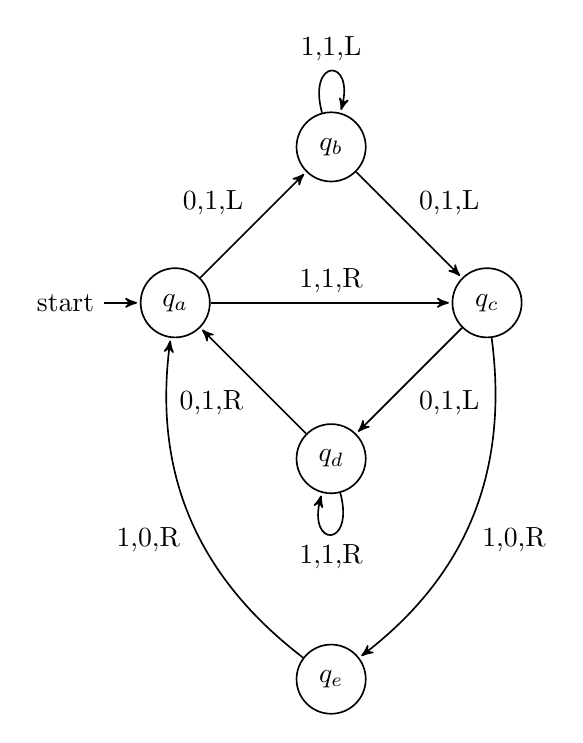
\begin{tikzpicture}[->,>=stealth',shorten >=1pt,auto,node distance=2.8cm,
                    semithick]
  % \tikzstyle{every state}=[fill=red,draw=none,text=white]
  % \tikzstyle{every state}=[fill=red,draw=none,text=white]

  \node[initial,state] (A)                    {$q_a$};
  \node[state]         (B) [above right of=A] {$q_b$};
  \node[state]         (D) [below right of=A] {$q_d$};
  \node[state]         (C) [below right of=B] {$q_c$};
  \node[state]         (E) [below of=D]       {$q_e$};

  \path (A) edge              node {0,1,L} (B)
            edge              node {1,1,R} (C)
        (B) edge [loop above] node {1,1,L} (B)
            edge              node {0,1,L} (C)
        (C) edge              node {0,1,L} (D)
            edge [bend left]  node {1,0,R} (E)
        (D) edge [loop below] node {1,1,R} (D)
            edge              node {0,1,R} (A)
        (E) edge [bend left]  node {1,0,R} (A);
\end{tikzpicture}

\begin{tikzpicture}
\begin{axis}[
    xlabel=degree (k),
  ylabel=Counts]
  \addplot table [col sep=comma]{orig.dat};
\addlegendentry{Orig}
  \addplot table [col sep=space]{ddphrg.dat};
\addlegendentry{PHRG}
%\addplot table [y=P, x=$Q_B$]{data.dat};
%\addlegendentry{$Q_B$ series}
%\addplot table [y=P, x=$Q_D$]{data.dat};
%\addlegendentry{$Q_D$ series}
\end{axis}
\end{tikzpicture}

% CDF https://matplotlib.org/examples/statistics/histogram_demo_cumulative.html
% http://stackoverflow.com/questions/24788200/calculate-the-cumulative-distribution-function-cdf-in-python
% https://docs.scipy.org/doc/scipy/reference/tutorial/stats.html
% http://www.math.pitt.edu/~lewicka/Semester_DiscrNetw_14/MNlecture22.pdf

\end{document}
